\section{Label Distribution}
We started by analyzing the distribution of the labels in the dataset, see Figure \ref{fig:label_dist}.
\begin{figure}[H]
    \vspace*{0.7cm}
    \centering
    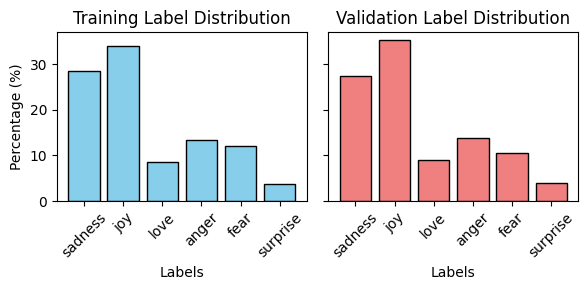
\includegraphics[width=0.5\textwidth]{figures/label_dist.png}
    \caption{Distribution of the labels in the dataset.}
    \label{fig:label_dist}
    \vspace*{0.7cm}
\end{figure}
From the figure, it is clear that the dataset is very unbalanced in the training set, with the majority of the tweets being labeled as joy or sadness. However, the validation set have more and less the same distribution of labels. Therefore, we expect the test set to have a similar distribution.

Of course, this unbalance in the training set will have an impact on the performance of the model, as sentences labeled as joy will be more less likely to be classified correctly. This is something we will have to take into account when evaluating the performance of the model.